\chapter{Comparison of Methods}

This chapter compares the performance of various methods used in the UAV navigation system, focusing on accuracy, runtime, and robustness. The evaluation includes feature detectors, local feature matchers, rotational and translational estimators, and optimization techniques. Each method is tested across multiple datasets to assess generalization and suitability for real-world UAV applications.

\section{Testing Setup}

This section outlines the framework used to evaluate the performance of the proposed UAV navigation methods. The evaluation focuses on three primary metrics: accuracy, runtime, and robustness. These metrics are critical to ensure that the navigation system can reliably operate under diverse and challenging conditions, reflecting real-world scenarios where the UAV may encounter varying environmental factors.

\subsection{Datasets}

Five distinct datasets were selected to rigorously evaluate the methods' generalization and performance across diverse environments. These datasets were captured using Google Earth and involved both translational and rotational movements, simulating typical UAV navigation tasks. Although the primary transformations were translation and rotation, perspective distortions and other subtle deformations were present due to the uneven terrain. Multiple methods with varying degrees of freedom were tested to implicitly estimate which of these transforms were significantly present. Each of the properties and choices were done to ensure the task was challenging but not impossible.

\textbf{General Properties of the Datasets:}
\begin{itemize}
    \item \textbf{Altitude:} Ranging from 5.5 to 6.5 km, constant within each dataset. This is standard for UAV navigation applications and ensures the ground is sufficiently planar.
    \item \textbf{Resolution:} 1920x972 pixels per image. This is the standard resolution in most applications. Stress tests were performed at lower resolutions.
    \item \textbf{Radial Movement Between Frames:} Approximately 600 pixels. This ensured sufficient overlap for a challenging but feasible task.
    \item \textbf{Number of Images per Dataset:} 15 images per dataset. This balances testing time and is sufficient to evaluate the methods' performance. 
\end{itemize}

The datasets used for testing were as follows:

\begin{itemize}
    \item \textbf{CITY1 and CITY2 (Cape Town):}  
    Both datasets were captured in Cape Town. \textbf{CITY1} includes both rotational and translational changes between frames, while \textbf{CITY2} focuses solely on translational movements. This distinction allows for isolated testing of performance under rotational stress.
    
    \item \textbf{ROCKY:}  
    This dataset covers rugged terrain with varying features, testing the methods' robustness in handling complex, uneven topographies.
    
    \item \textbf{DESERT and AMAZON:}  
    These datasets are characterized by sparse, repetitive patterns, making it challenging even for human observers to distinguish differences between frames. They present significant difficulty for feature extraction and matching.
\end{itemize}

Examples of the datasets are shown below:

\begin{figure}[H]
    \centering
    \begin{minipage}{0.45\textwidth}
        \centering
        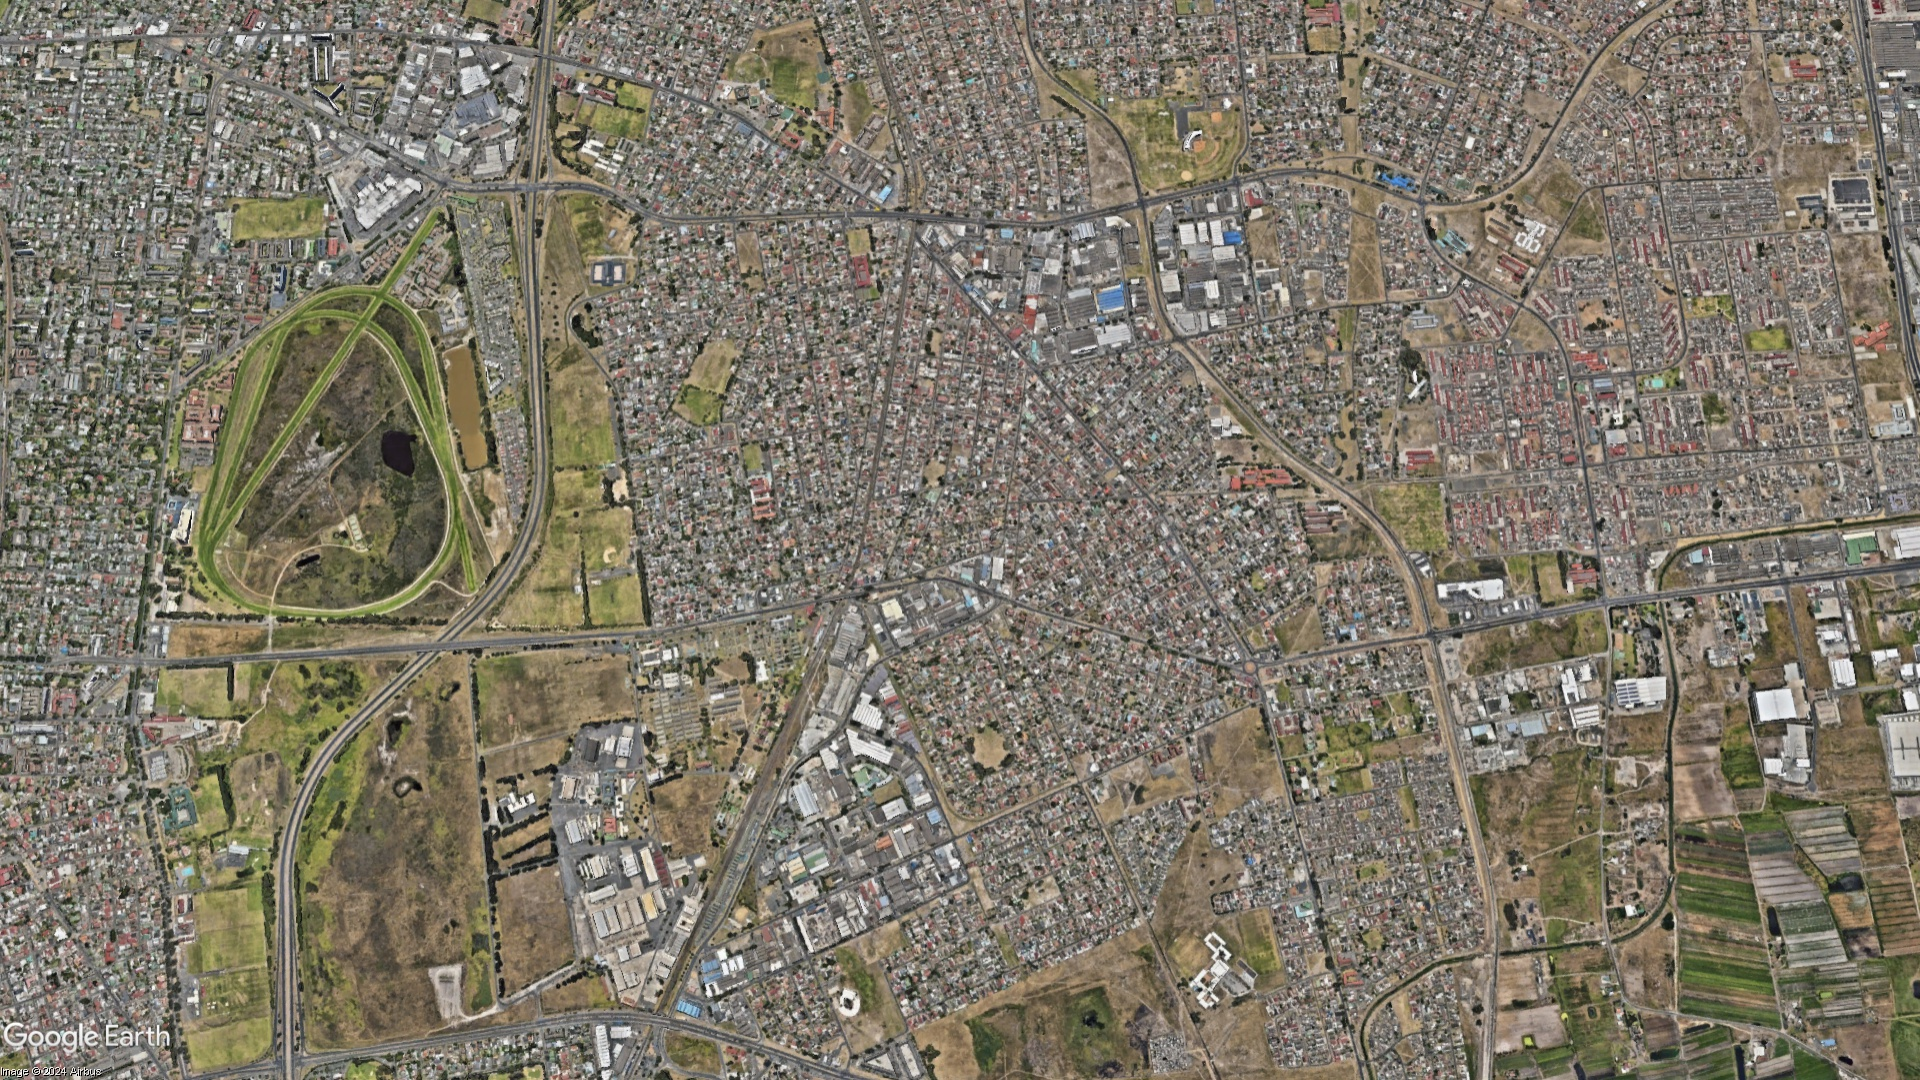
\includegraphics[width=\textwidth]{./Chapter 4/DEMODATASETS/CITY1.jpg}
        \caption{Examples of the CITY1 and CITY2 Datasets}
        \label{fig:CITY12}
    \end{minipage}\hfill
    \begin{minipage}{0.45\textwidth}
        \centering
        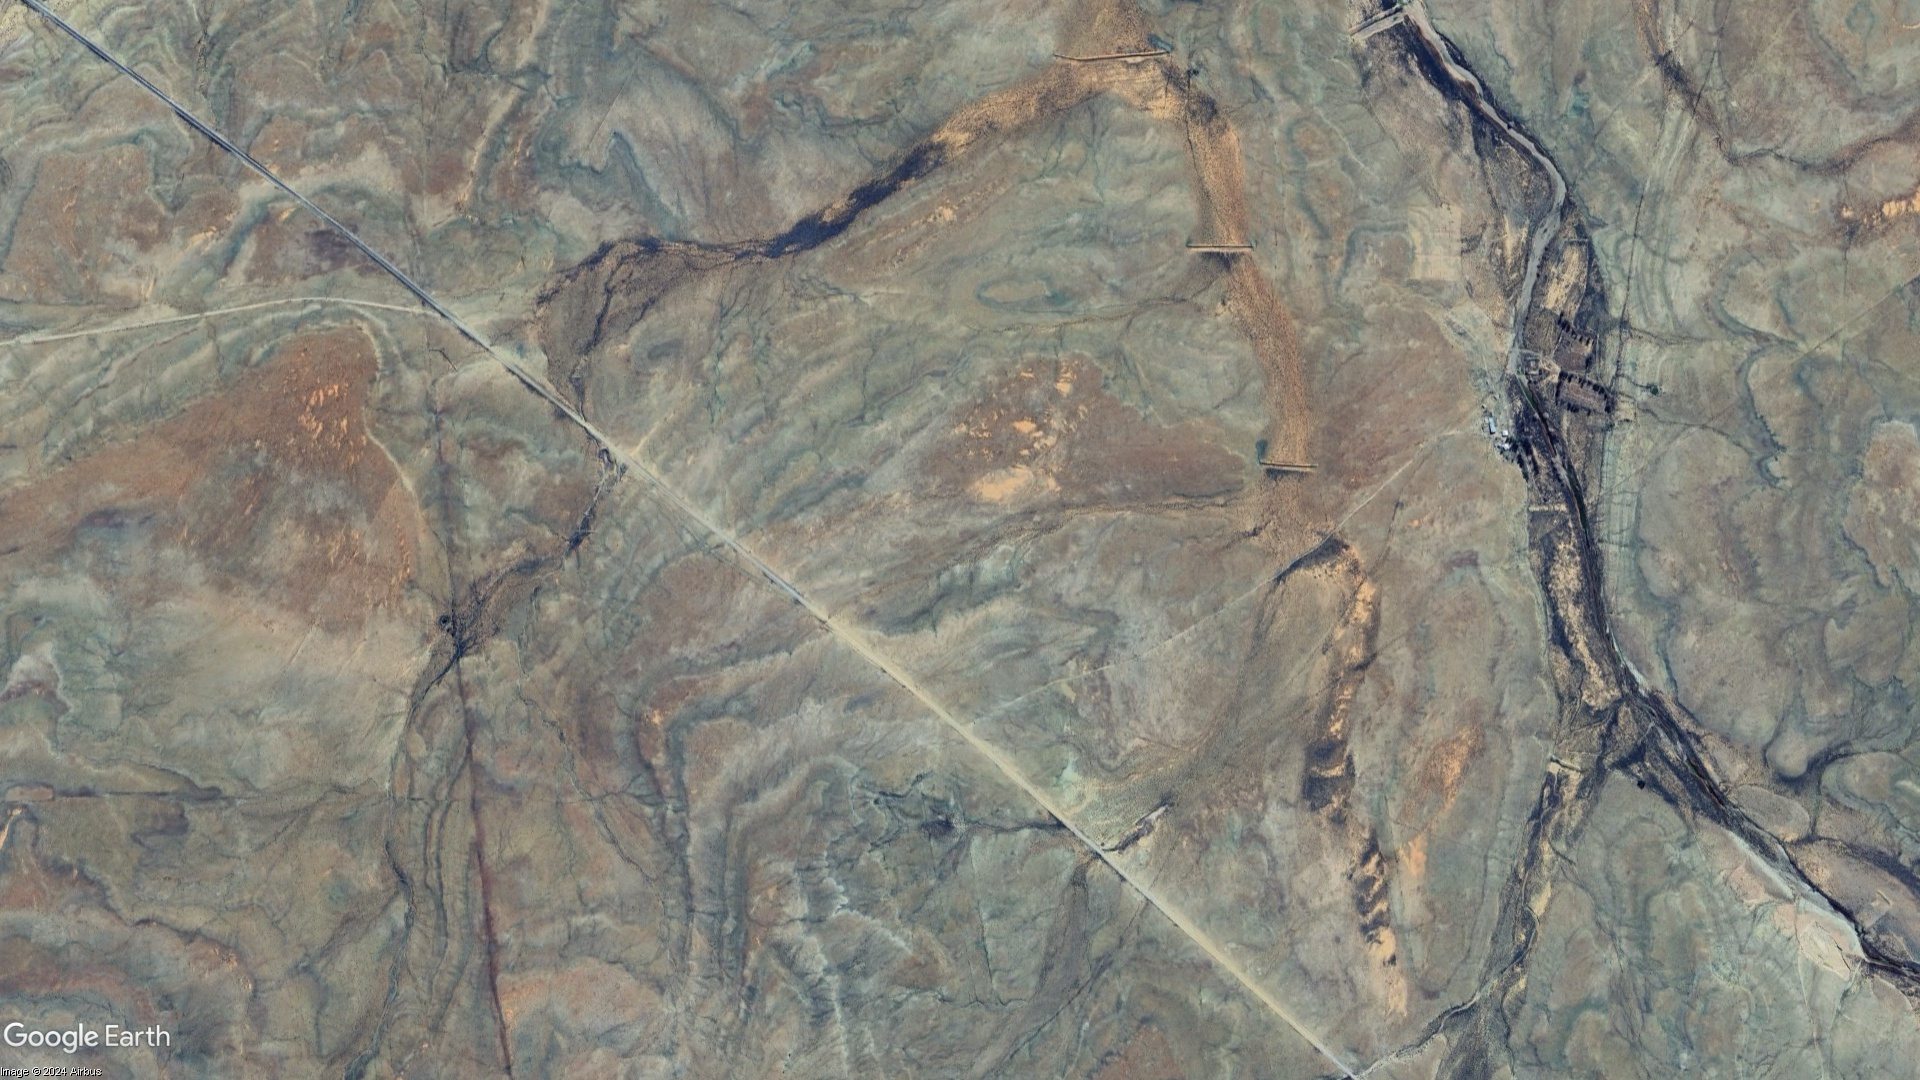
\includegraphics[width=\textwidth]{./Chapter 4/DEMODATASETS/ROCKY.jpg}
        \caption{Example of the ROCKY Dataset}
        \label{fig:ROCKY}
    \end{minipage}
    
    \vspace{0.5cm} % Add some vertical space between rows
    
    \begin{minipage}{0.45\textwidth}
        \centering
        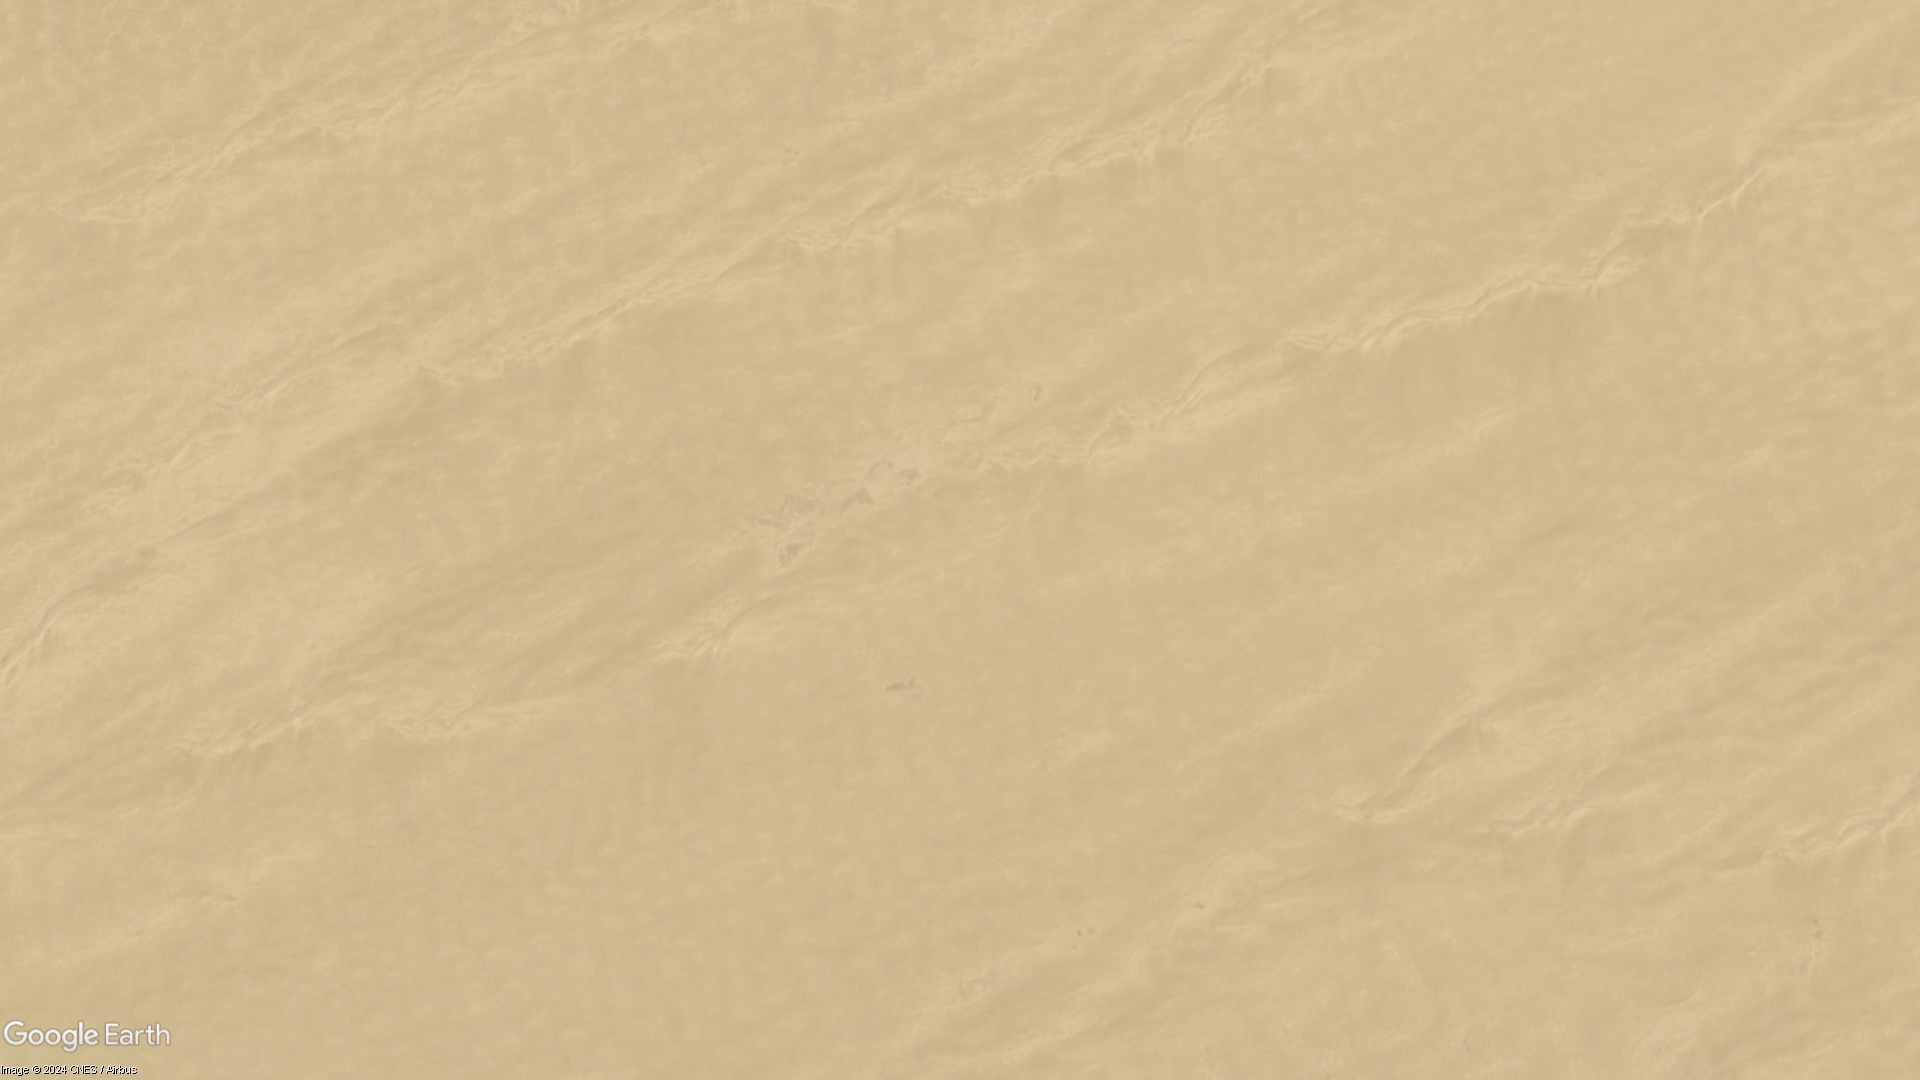
\includegraphics[width=\textwidth]{./Chapter 4/DEMODATASETS/DESERT1.jpg}
        \caption{Example of the DESERT Dataset}
        \label{fig:DESERT}
    \end{minipage}\hfill
    \begin{minipage}{0.45\textwidth}
        \centering
        
\includegraphics[width=\textwidth]{./Chapter 4/DEMODATASETS/AMAZON.jpg}
        \caption{Example of the AMAZON Dataset}
        \label{fig:AMAZON}
    \end{minipage}
    
    \caption{Overview of Datasets}
    \label{fig:Datasets}
\end{figure}



\subsection{Testing Structure}

Each method is subjected to rigorous testing based on the following criteria:

\begin{itemize}
    \item \textbf{Accuracy}: Evaluated using the Root Mean Square Error (RMSE) of GPS estimations, accuracy assessments focus on the end error. This is justified because outputs—whether images or degrees—propagate through the pipeline, meaning any errors or poor choices are ultimately reflected in the final GPS error.
    \item \textbf{Runtime}: The entire system runtime per dataset is assessed to evaluate the computational efficiency of each method. Efficient runtimes are crucial for real-time UAV applications, as delays—combined with pilot and UAV response times—can result in consistently missing the target and failing to follow the intended path. As before, runtime may propagate through the system, and therefore the runtime per line is not necessarily indicative of better performance; Runtime per line is not tested. 
    \item \textbf{Robustness}: Tested to verify each method's stability under parameter variations and challenging conditions. Robust methods maintain consistent performance despite environmental or parameter changes, ensuring reliable UAV navigation across different scenarios.
\end{itemize}

This structured testing approach ensures that each component of the UAV navigation system is thoroughly evaluated, facilitating the selection of methods that deliver optimal performance across all critical metrics.

\subsection{Parameters}  
Parameters were held constant across tests and chosen to ensure optimal performance across methods. The focus was not on selecting the absolute best parameter set, as this was not relevant for inter-method testing; rather, the goal was to minimize bias while allowing each method to perform effectively. For instance, multiple methods were tested within a single runtime to enhance testing speed without compromising the integrity of the inter-method comparisons. The takeaway here is to avoid interpreting results objectively, as they do not reflect the realistic and overall performance of the system.



\section{Feature Detectors}

This section presents the evaluation results of three feature detectors: ORB, AKAZE, and SuperPoint with LightGlue. The results from these tests informed the selection of the most appropriate detector and threshold parameters for the crude and dense layer of keypoints.

\subsection{Accuracy and Runtime}

Figure \ref{fig:rmse_detectors} and Figure \ref{fig:runtime_detectors} present the RMSE and runtime values for each feature detector across different datasets. AKAZE, utilizing dynamic keypoint targeting, demonstrated the highest accuracy across all datasets while maintaining reasonable runtime. SuperPoint recorded the highest RMSE values, particularly in challenging datasets such as ROCKY and AMAZON, indicating its limited generalizability across diverse environments. Meanwhile, ORB proved to be the most efficient detector, making it suitable for applications requiring fast processing. SuperPoint demonstrated the longest runtimes across all datasets, highlighting its limited applicability for time-sensitive applications unless optimized with GPU acceleration.

\begin{figure}[H]
    \centering
    \begin{minipage}{0.45\textwidth}
        \centering
        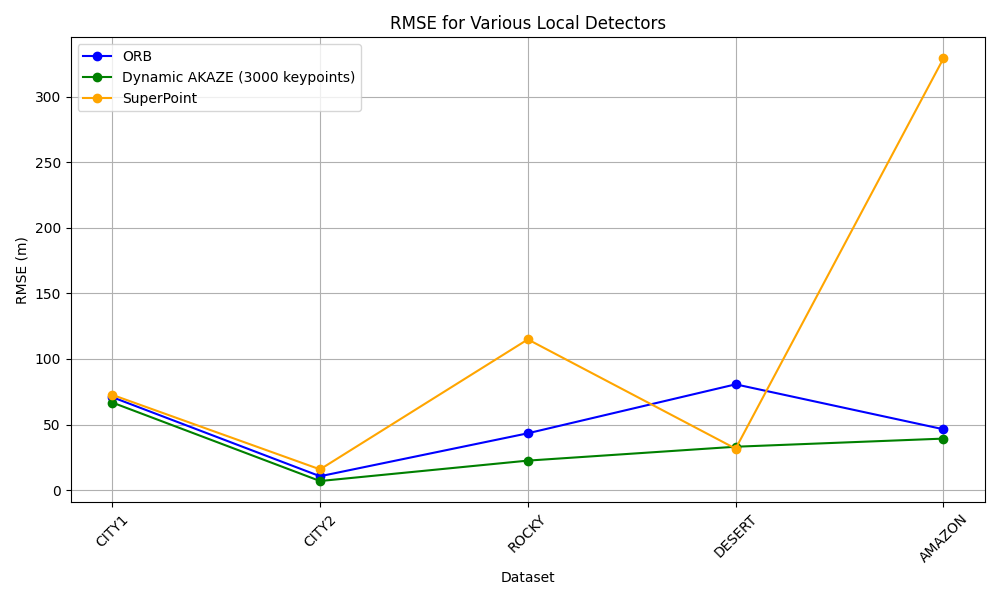
\includegraphics[width=\textwidth]{./Chapter 4/testresults/rmse_detectors.png}
        \caption{RMSE for Various Local Detectors}
        \label{fig:rmse_detectors}
    \end{minipage}\hfill
    \begin{minipage}{0.45\textwidth}
        \centering
        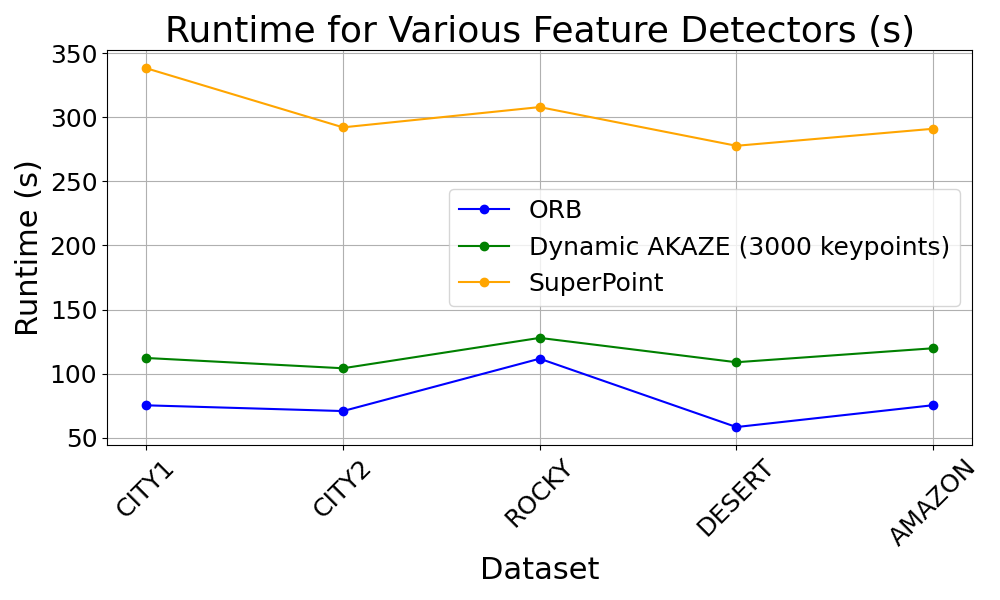
\includegraphics[width=\textwidth]{./Chapter 4/testresults/runtime_detectors.png}
        \caption{Runtime for Various Local Detectors}
        \label{fig:runtime_detectors}
    \end{minipage}
    \caption{RMSE and Runtime Comparison for ORB, AKAZE, and SuperPoint Across Datasets}
    \label{fig:rmse_runtime_detectors}
\end{figure}


\subsubsection{Robustness}

When paired with keypoint targeting, all features obtained the same number of keypoints across datasets. However, the quality of the keypoints varied significantly. However, AKAZE managed to consistently deliver less noisy keypoints, making it the most robust detector across all datasets. 

\subsection{Final Selection of Feature Detectors}

Based on the comprehensive evaluation, the following detectors were selected for the respective stages of the UAV navigation system:

\begin{itemize}
    \item \textbf{Crude Layer (Initial Detection)}: \textbf{ORB} was chosen for the crude layer due to its balance of accuracy and efficiency with 2500 keypoints. 
    
    \item \textbf{Dense Layer (Refined Detection)}: \textbf{Dynamic AKAZE} with 3000 keypoints was selected for the dense layer due to its consistent performance and robustness. This detector complements the crude layer by refining feature extraction and enhancing the system's accuracy.
\end{itemize}


\section{Local Feature Matchers}

This section evaluates two prominent local matchers, BFMatcher and FLANN, within the context of a UAV navigation system. 

\subsection{Accuracy and Runtime Evaluation}

Figure \ref{fig:rmse_flann_bf} presents the Root Mean Squared Error (RMSE) in GPS values for BFMatcher and FLANN across different datasets. The results indicate that while BFMatcher achieves slightly better accuracy in certain cases, FLANN remains highly competitive with only marginally higher RMSE values.

Figure \ref{fig:runtime_flann_bf} shows the runtime comparison for BFMatcher and FLANN across different datasets. FLANN consistently outperforms BFMatcher in terms of speed, with significantly lower execution times across all datasets.

\begin{figure}[H]
    \centering
    \begin{minipage}{0.45\textwidth}
        \centering
        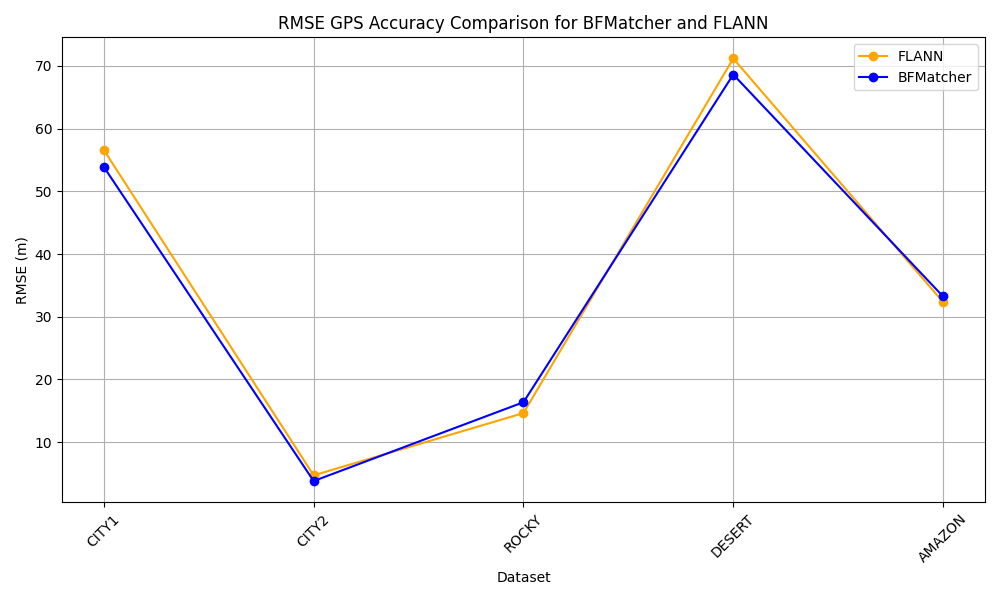
\includegraphics[width=\textwidth]{./Chapter 4/testresults/rmse_flann_bf.png}
        \caption{RMSE GPS Accuracy for BFMatcher and FLANN}
        \label{fig:rmse_flann_bf}
    \end{minipage}\hfill
    \begin{minipage}{0.45\textwidth}
        \centering
        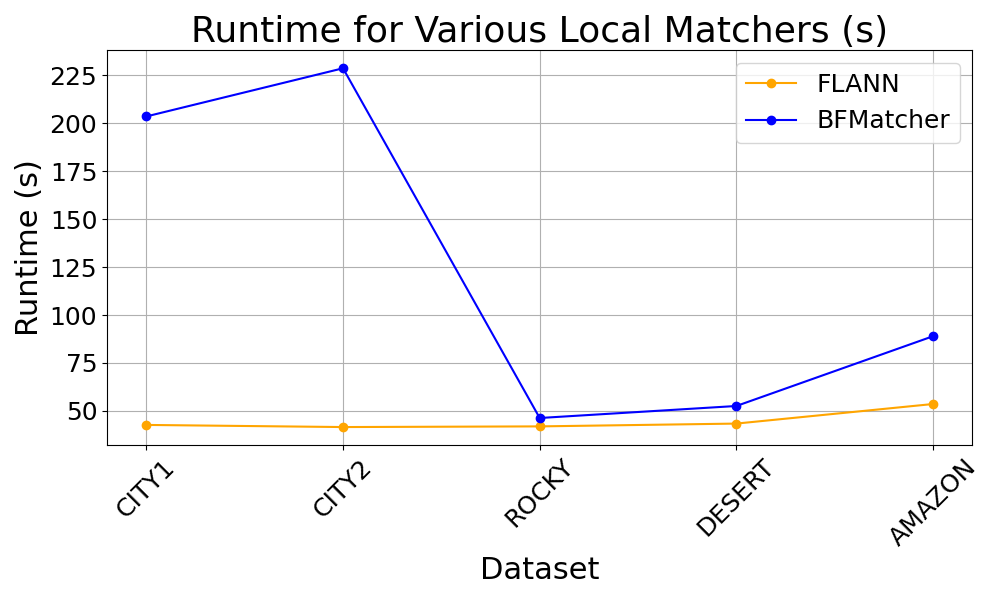
\includegraphics[width=\textwidth]{./Chapter 4/testresults/runtime_flann_bf.png}
        \caption{Runtime Comparison for BFMatcher and FLANN}
        \label{fig:runtime_flann_bf}
    \end{minipage}
\end{figure}



\subsection{Robustness Under Varying Detector Thresholds}

Figure \ref{fig:divergence_plot} depicts the divergence in RMSE GPS error between FLANN and BFMatcher as the number of keypoints increases. Positive values indicate that BFMatcher outperforms FLANN, while negative values suggest FLANN performs better. The plot demonstrates the convergence of both matchers' accuracy as the number of keypoints increases, with FLANN generally maintaining slightly higher RMSE values than BFMatcher. Note that outliers are present, indicating instances where FLANN achieves better accuracy than BFMatcher. This is attributed to FLANN's approximate matching, paired with a static Lowe's ratio threshold, which may preserve valid matches that BFMatcher might discard.

\begin{figure}[H]
    \centering
    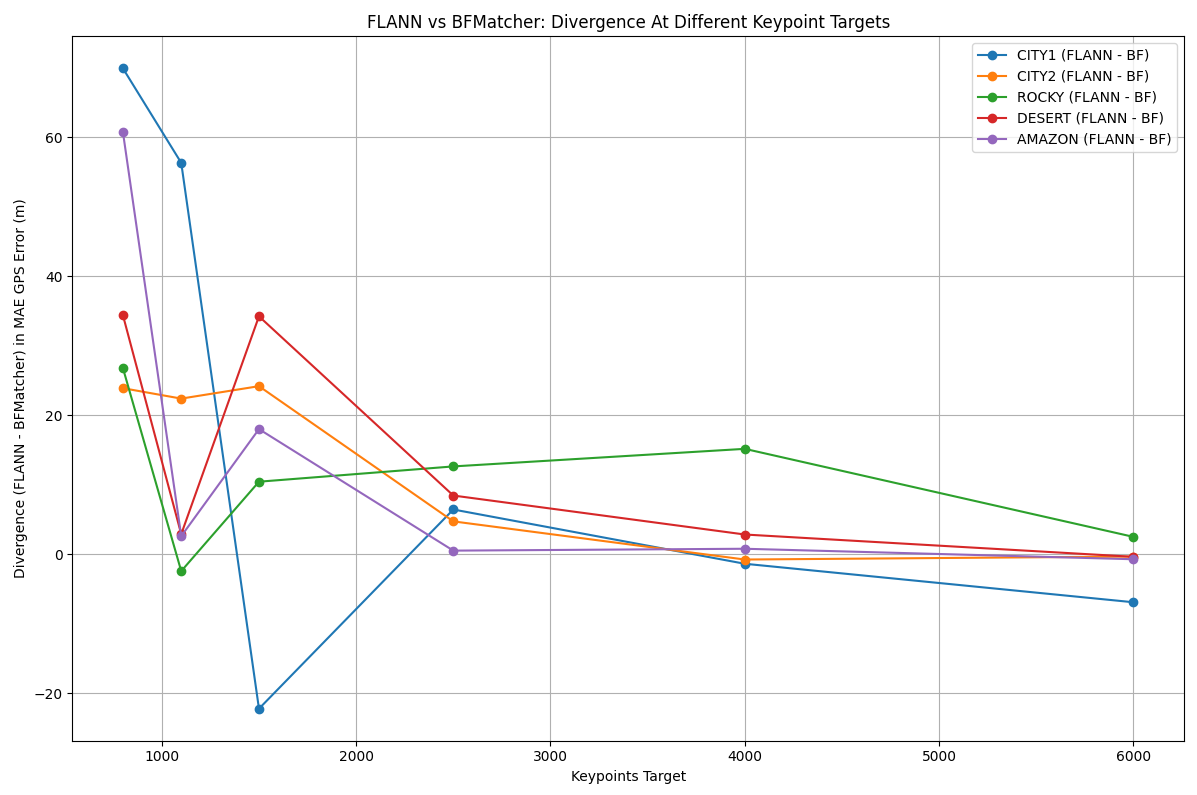
\includegraphics[width=0.8\textwidth]{./Graphs/Divergence_BF_FLANN_KPS.png}
    \caption{Divergence in RMSE GPS Error Between FLANN and BFMatcher Across Keypoint Targets}
    \label{fig:divergence_plot} 
\end{figure}

\subsection{Final Selection of Local Feature Matcher}

Based on the comprehensive evaluation of accuracy, runtime, and robustness, FLANN emerges as the optimal choice for the UAV navigation system. FLANN offers significantly faster runtimes and better scalability while maintaining comparable accuracy to BFMatcher. This makes FLANN highly suitable for real-time applications where computational efficiency is paramount.


\section{Planar Transform Estimators}

This section evaluates the performance of four planar transformation estimation methods: Partial Affine 2D (Rigid Transform plus minor Scaling), Affine 2D, Homography, and Rigid Transform Via SVD. As noted in section \ref{sec:testing_shortlist}, the accuracy of the method when used for rotational and translational estimates were seen to be comparatively equivalent. Thus, methods were tested for their combined influence on the accuracy on the transformation estimates, as viewed through the GPS error. For these tests, RANSAC was used on all methods, except the Rigid Transform Via SVD, to filter outliers.

\subsection{Accuracy and Runtime Evaluation}

Figure \ref{fig:rmse_runtime_comparison_rotestim} summarizes the RMSE and runtime values across datasets for each rotational estimator method. From the results, it is clear that each method exhibits strengths in different datasets. However, the Rigid SVD method and Partial Affine 2D consistently emerge as the most accurate methods. This implies that the Rigid SVD transform provides the most stable and accurate estimate of the rotational and translational components of the UAV's movement. The Rigid SVD method slightly outperforms Partial Affine 2D in most datasets, attributed to its strict rigid transformation alignment with dataset characteristics.

The runtime results, shown in \ref{fig:rmse_runtime_comparison_rotestim}, are influenced by the degrees of freedom in each method, with rigid-based transforms demonstrating the best performance across datasets. SVD proves the fastest due to its lack of iterative optimization.


\begin{figure}[H]
    \centering
    \begin{minipage}{0.45\textwidth}
        \centering
        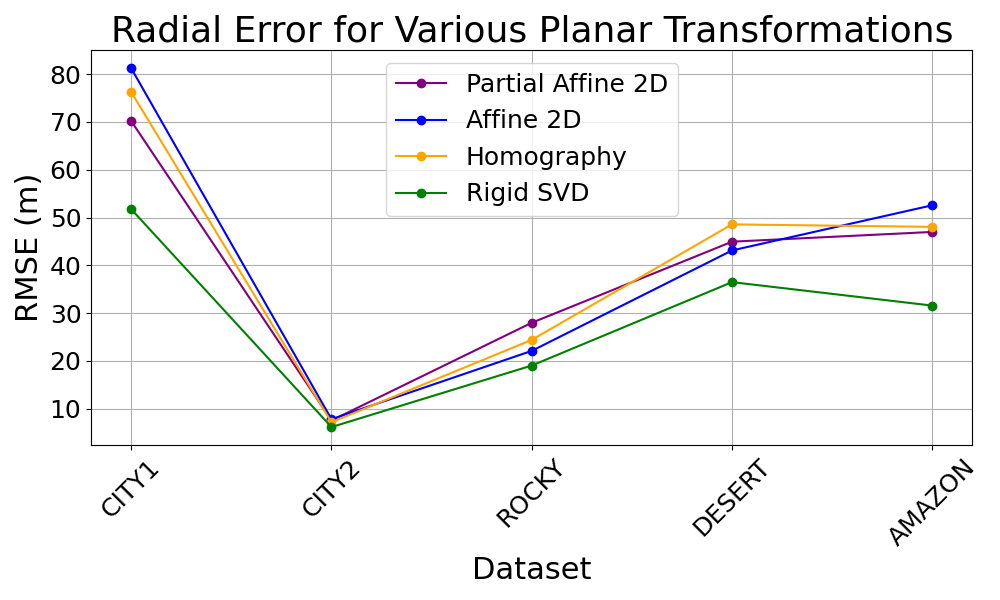
\includegraphics[width=\textwidth]{./Chapter 4/testresults/rmse_planar_estimators.png}
        \caption{RMSE Comparison Across Datasets for Planar Transform Estimators}
    \end{minipage}\hfill
    \begin{minipage}{0.45\textwidth}
        \centering
        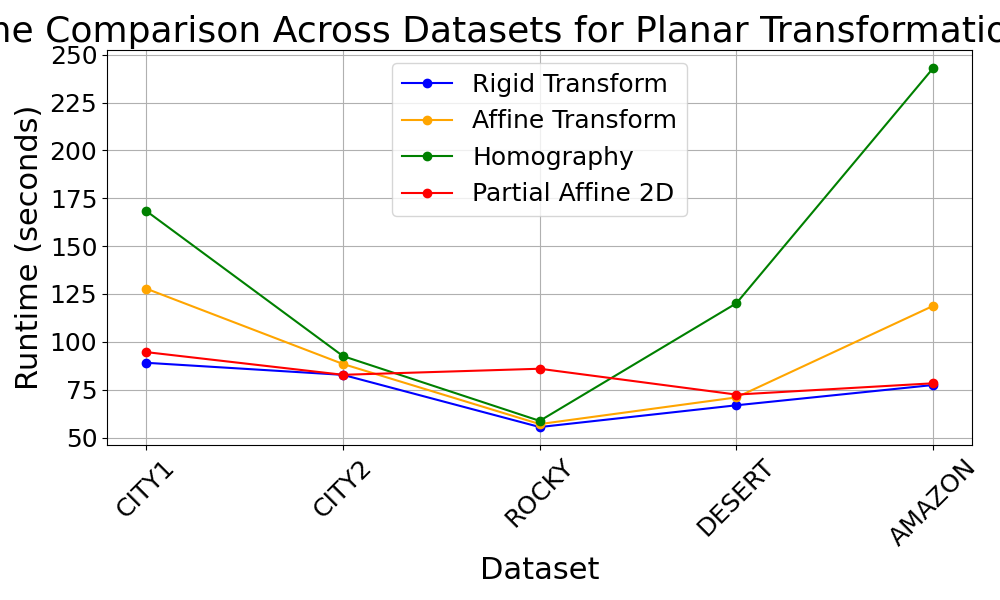
\includegraphics[width=\textwidth]{./Chapter 4/testresults/runtime_planar_estimators.png}
        \caption{Runtime Comparison Across Datasets for Planar Transform Estimators}
    \end{minipage}
    \caption{RMSE and Runtime Comparison Across Datasets for Planar Transform Estimators}
    \label{fig:rmse_runtime_comparison_rotestim}
\end{figure}
   
    

\subsection{Robustness Testing}

Robustness testing assessed each method's sensitivity to parameter variations, including Lowe’s ratio and keypoint detectors and their corresponding detection thresholds. This evaluation was essential to determine the performance consistency of each method under different challenging conditions. For the sake of brevity, the results are omitted; The recorded observations are summarized below.


\textbf{Observations:}  
\begin{itemize}
    \item \textbf{Parameter Sensitivity:} All methods were highly robust to parameter variations, maintaining consistent performance across different settings.
    \item \textbf{Best Robustness:} The Rigid SVD Transform exhibited the highest robustness across all parameters, especially at low keypoint counts.

\end{itemize}

\subsection{Final Selection of Transformational Estimator}

Based on the comprehensive evaluation of accuracy, runtime, and robustness, the rigid transform by SVD emerged as the most suitable rotational estimator for the UAV navigation system. It demonstrated the lowest combined radial RMSE in GPS across all datasets, the fastest runtime, and high robustness due to its precise match to the degrees of freedom in the datasets. Further, it required no parameter tuning, making it highly suitable for real-time UAV applications.





\section{Image Similarity Estimators}

Accurate image similarity estimation, or global matching, is essential for UAV navigation systems to choose reasonable images to compare to. They should ensure accuracy and efficiency while maintaining robustness against small rotational offsets. 

\subsection{Accuracy Evaluation}

\subsection{Accuracy and Runtime Evaluation}

Naturally, the appropriateness of the choice of best match is implicitly passed through to subsequent stages and realized as an error in GPS estimations. Figure \ref{fig:rmse_global_matching} summarizes the RMSE values (in meters) for Local Retrofit, Cross Correlation, Histogram, and SSIM. The results indicate that the Histogram technique consistently achieved the lowest RMSE across most datasets, followed by Cross Correlation and SSIM. The Local Retrofit method recorded the highest RMSE values, especially in the DESERT dataset, indicating poor generalizability and higher complexity; It was excluded from further analysis.

Figure \ref{fig:runtime_global_matching} compares the computational efficiency of each global matching technique across the five datasets. The Histogram technique demonstrated the fastest runtimes, followed closely by Cross Correlation. SSIM exhibited the longest runtimes, particularly in the AMAZON and DESERT datasets, rendering it less suitable for real-time applications.


\begin{figure}[H]
    \centering
    \begin{minipage}{0.45\textwidth}
        \centering
        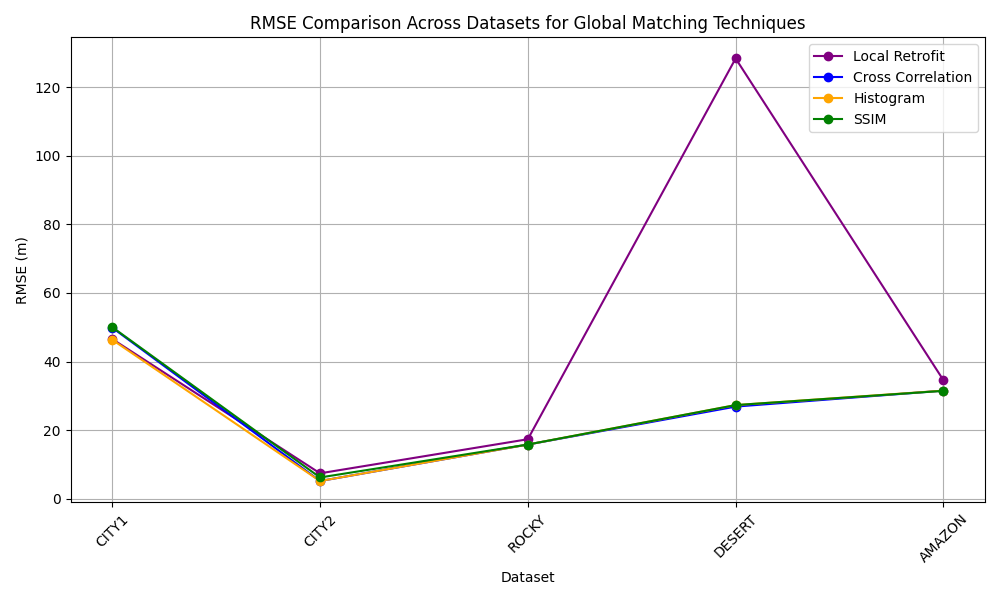
\includegraphics[width=\textwidth]{./Chapter 4/testresults/rmse_global_matching.png}
        \caption{RMSE Comparison Across Datasets for Global Matching Techniques}
        \label{fig:rmse_global_matching}
    \end{minipage}\hfill
    \begin{minipage}{0.45\textwidth}
        \centering
        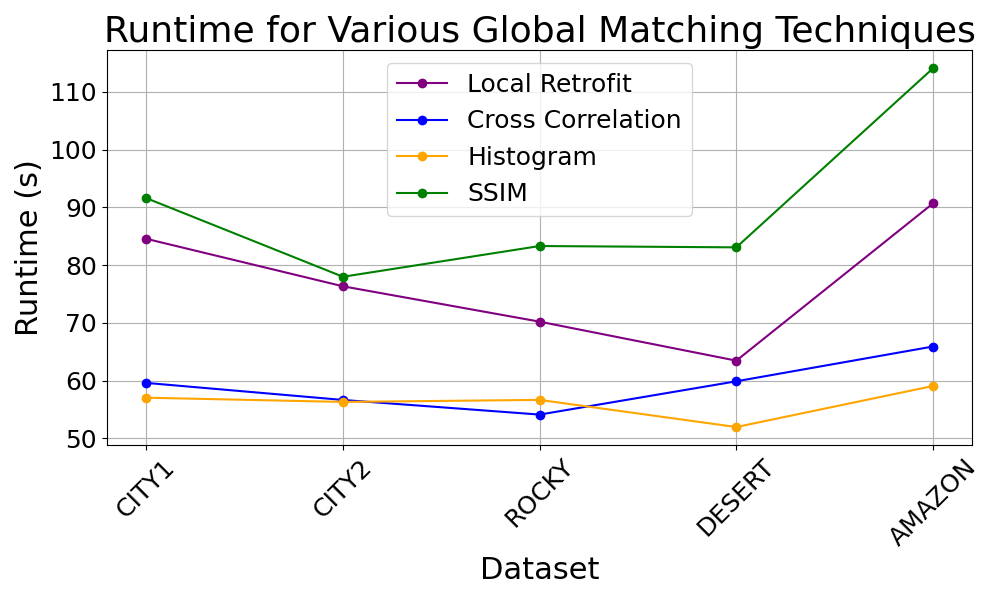
\includegraphics[width=\textwidth]{./Chapter 4/testresults/runtime_global_matching.png}
        \caption{Runtime Comparison Across Datasets for Global Matching Techniques}
        \label{fig:runtime_global_matching}
    \end{minipage}
\end{figure}

\subsection{Robustness to Rotational Offsets}

Robustness testing evaluated each global matching technique's sensitivity to a 5- and 10-degree rotational offset. All matchers that made it this far saw no change in choice combination below a 5-degree offset. The resultant percentage deviation under a 10-degree offset is shown in Figure \ref{fig:percentage_change_comparison_methods}. 
Cross-correlation was the most robust, with the lowest percentage change in GPS error, from its prior estimate, across all datasets. Histogram and SSIM exhibited moderate robustness, while SSIM demonstrated the highest maximum error and variability. However, the ability of all matchers to maintain equivalent performance under offsets of up to 5 degrees suggests that they are all extremely robust to small rotational misalignments; This allows for prioritization of efficiency in the sections outputting the rotational estimate to this stage.

\begin{figure}[H]
    \centering
    \begin{minipage}{0.45\textwidth}
        \centering
        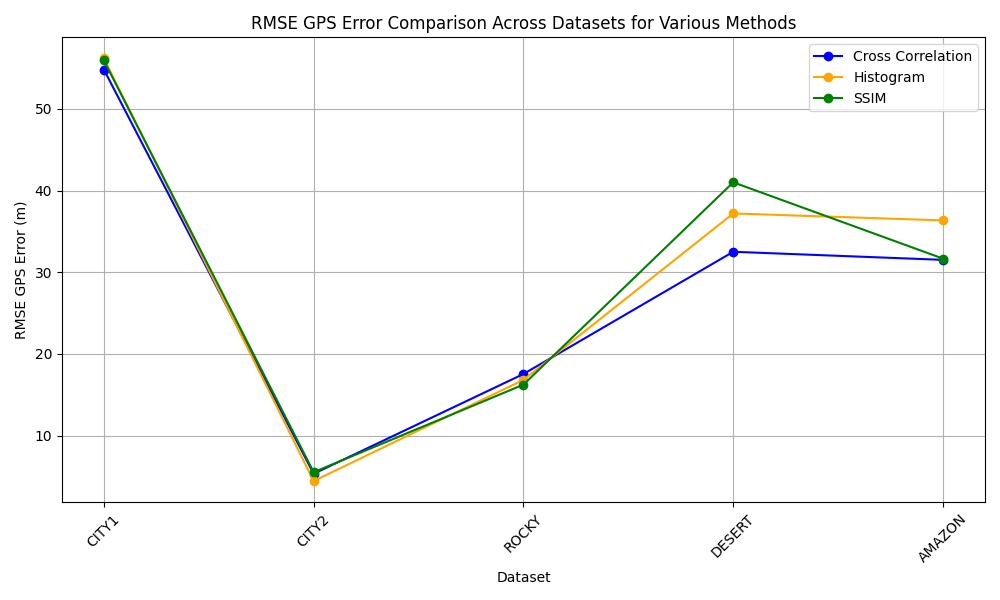
\includegraphics[width=\textwidth]{./Chapter 4/testresults/rmse_comparison_methods.png}
        \caption{RMSE GPS Error Comparison Across Datasets for Various Methods}
        \label{fig:rmse_comparison_methods}
    \end{minipage}\hfill
    \begin{minipage}{0.45\textwidth}
        \centering
        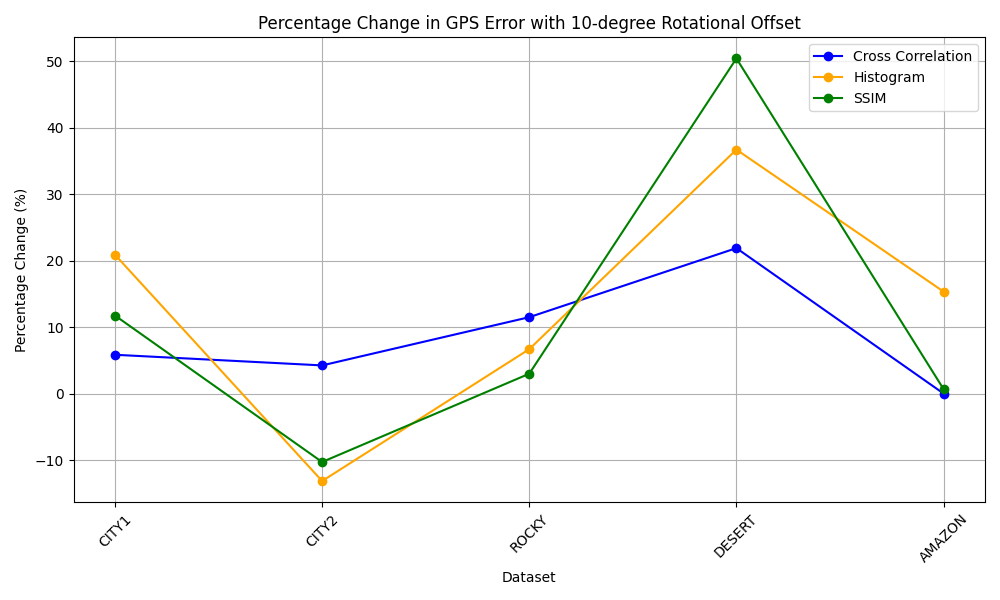
\includegraphics[width=\textwidth]{./Chapter 4/testresults/percentage_change_comparison_methods.png}
        \caption{Percentage Change in GPS Error with 10-degree Rotational Offset}
        \label{fig:percentage_change_comparison_methods}
    \end{minipage}
\end{figure}



\subsection{Final Selection of Global Matching Technique}

Based on the comprehensive evaluation of accuracy, runtime, and robustness, the \textbf{Histogram} technique is identified and chosen as the most suitable global matching method for the system. Histogram consistently provided superior performance in terms of both RMSE and runtime, whilst maintaining sufficient robustness to rotational error. 




\section{Optimization Techniques}

This section outlines the selected optimization methods employed to improve the performance of the UAV navigation system. The optimization techniques focus on filtering matches between images to balance noise and stability in the point sets. 


\subsection{Planar Transform Outlier Rejection Methods}

Two outlier rejection methods, LMEDS (Least Median of Squares) and RANSAC (Random Sample Consensus), were evaluated for match filtration. Both methods performed near equivalently, with LMEDS displaying a slightly lower mean deviation. LMEDS was also significantly faster than RANSAC, making it the preferred choice for planar transform outlier rejection. The results are summarized in Figure \ref{fig:rmse_comparisonlmeds} and Figure \ref{fig:runtime_comparisonlmeds}.

\begin{figure}[H]
    \centering
    \begin{minipage}{0.45\textwidth}
        \centering
        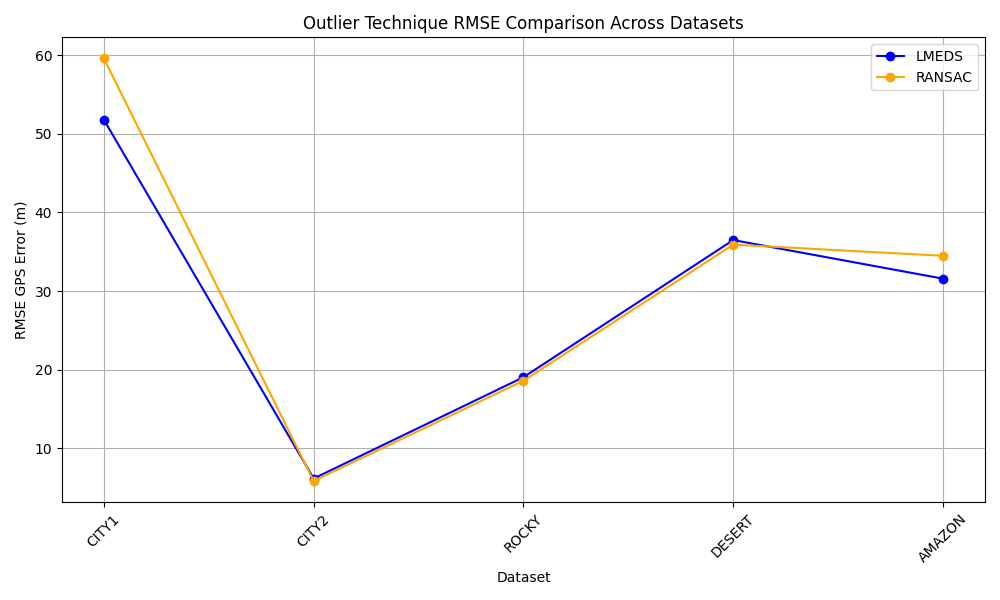
\includegraphics[width=\textwidth]{./Chapter 4/testresults/ransaclmedsrmse.png}
        \caption{Radial GPS RMSE Comparison Across Datasets for LMEDS and RANSAC}
        \label{fig:rmse_comparisonlmeds}
    \end{minipage}\hfill
    \begin{minipage}{0.45\textwidth}
        \centering
        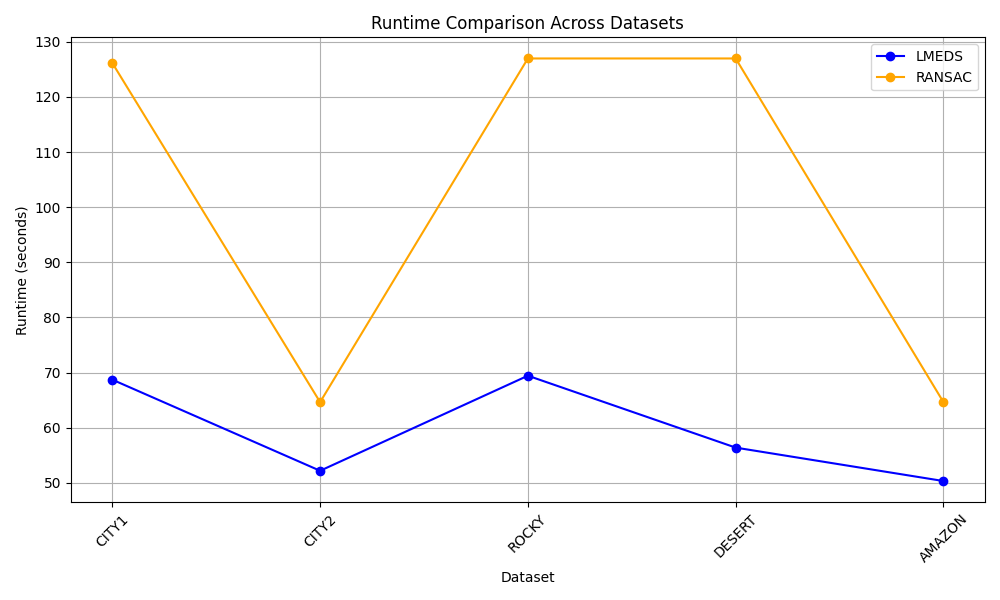
\includegraphics[width=\textwidth]{./Chapter 4/testresults/ransaclmedsruntime.png}
        \caption{Runtime Comparison Across Datasets for LMEDS and RANSAC}
        \label{fig:runtime_comparisonlmeds}
    \end{minipage}
\end{figure}



\subsection{Lowe's Ratio Test}

Lowe's ratio test was employed to filter keypoint matches by comparing the distance of the best match to the second-best match. A static threshold proved inadequate for generalizing across diverse datasets, leading to inconsistent accuracy. To enhance robustness, a dynamic thresholding approach was implemented. The initial Lowe's ratio was set low and incrementally increased until a predetermined number of matches was achieved. The parameters chosen were 0.5 to 0.7 for the initial Lowe's ratio, 0.025 to 0.1 for the step size, 10 to 30 for the maximum iterations, and 2000 to 3000 for the minimum matches. These parameters were selected to balance generalization and match quality, ensuring a sufficient number of reliable matches without compromising accuracy. The dynamic Lowe's ratio filtering method was found to significantly enhance the quality of matches, improving the overall accuracy of the system.


\subsection{Standard Deviation Filtering}

Standard Deviation Filtering was applied to both the magnitudes and angles of the match points. It was effective when coupled with the median, for robust outlier rejection, and applied to the vector using a standard deviation in the range of 1 and 3. This balanced stability and the exclusion of false positives. Standard Deviation Filtering was found to significantly improve the quality and consistency of matches, enhancing the overall accuracy of the system.

\subsection{{N-Match or Absolute Thresholding}}
These approaches leveraged fixed number or descriptor distance thresholds to filter matches. However, without relativity to the density and quality of keypoints, empirical tests revealed that these methods added instability to the system. They either had no meaningful effect or removed too many matches, leading to loss of accuracy. The thresholds were deemed too sensitive for generalized applications. 



\section{Summary}
The following methods were selected based on the comprehensive evaluation of accuracy, runtime, and robustness across diverse datasets:

\begin{itemize}
    \item \textbf{Feature Detectors:} ORB for the crude layer and Dynamic AKAZE for the dense layer.
    \item \textbf{Local Feature Matcher:} FLANN for its superior runtime and scalability.
    \item \textbf{Transformational Estimator:} Rigid Transform SVD for its high accuracy, fast runtime, and robustness.
    \item \textbf{Image Similarity Estimator:} Histogram for its superior accuracy and runtime.
    \item \textbf{Optimization Techniques:} Dynamic Lowe's filtering and Standard Deviation Filtering for enhanced match quality and consistency; LMEDS was not included due to prior choices of methods not requiring it.
\end{itemize}